\subsection{Стохастические диаграммы}

    Далее представлено влияние случайного возмущения на бифуркационных диаграммах для разных видов шума. На рисунках \ref{bifurcation_x_0_2_a_1_compare_alpha_noise}, \ref{bifurcation_x_0_2_a_1_compare_beta_noise} и \ref{bifurcation_x_0_2_a_1_compare_additional_noise} представлены графики бифуркационных диаграмм для моделей (\ref{alpha_chaos}), (\ref{beta_chaos}) и (\ref{additive_chaos}) соответсвенно. Во всех моделях зафиксировано значение параметра \(\alpha = 1\). На каждом графике, так же как и в исходной модели, существует участок равновесия, участки с циклами и участок с хаотическим поведением системы. От вида и интенсивности шума зависит то, насколько выделены участки с регулярной динамикой.

    Видно, что модель с \(\alpha\)-шум сохранят бифуркационную структуру лучше, чем модель с \(\beta\)-шумом и с аддитивным шумом.

    \begin{figure}
        \centering
        \subfloat[для модели (\ref{origin}) (без шума)]{
            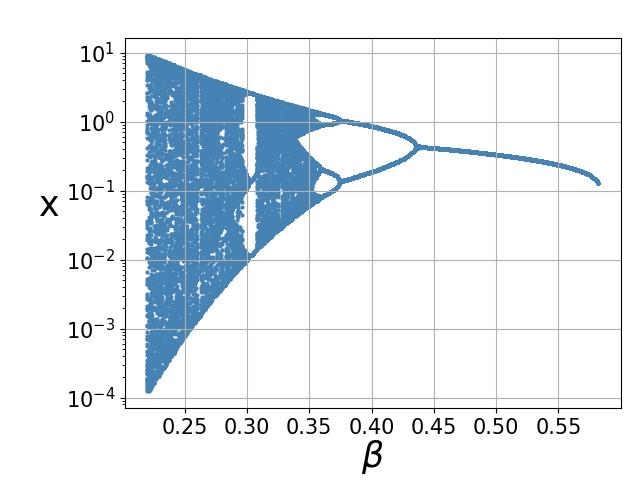
\includegraphics[width=0.5\textwidth]{stochastic/images/bifurcation_x_0_2_a_1_compare_no_noise.jpg}
            \label{bifurcation_x_0_2_a_1_compare_no_noise}
        }  
        \subfloat[для модели (\ref{alpha_chaos}) (с \(\alpha\)-шумом)]{
            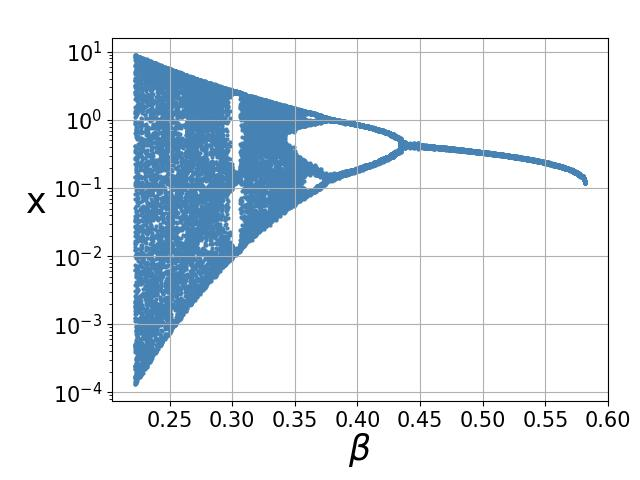
\includegraphics[width=0.5\textwidth]{stochastic/images/bifurcation_x_0_2_a_1_compare_alpha_noise.jpg}
            \label{bifurcation_x_0_2_a_1_compare_alpha_noise}
        }
        
        \subfloat[для модели (\ref{beta_chaos}) (с \(\beta\)-шумом)]{
            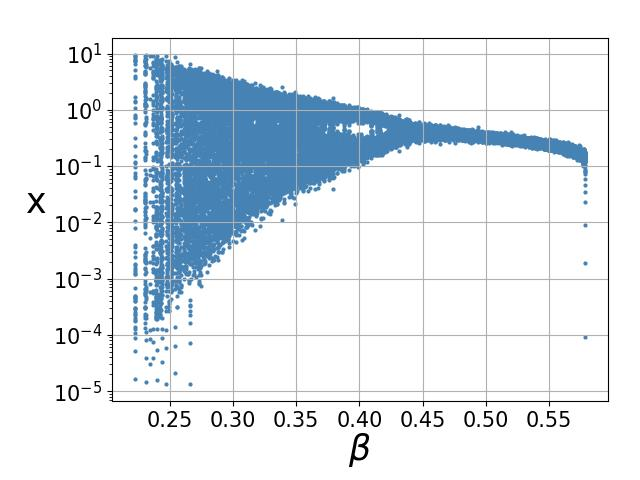
\includegraphics[width=0.5\textwidth]{stochastic/images/bifurcation_x_0_2_a_1_compare_beta_noise.jpg}
            \label{bifurcation_x_0_2_a_1_compare_beta_noise}
        }
        \subfloat[для модели (\ref{additive_chaos}) (с аддитивным шумом)]{
            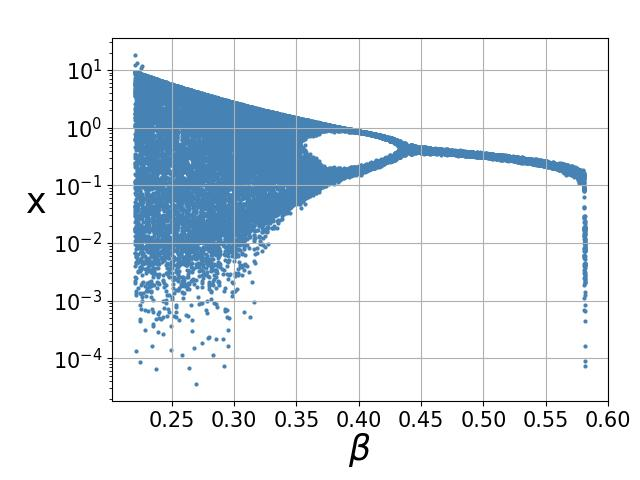
\includegraphics[width=0.5\textwidth]{stochastic/images/bifurcation_x_0_2_a_1_compare_additional_noise.jpg}
            \label{bifurcation_x_0_2_a_1_compare_additional_noise}
        }
            
        \captionsetup{justification=centering}
        \caption{Бифуркационная диаграмма при \(\varepsilon = 0.01\)}
    \end{figure}

    % \begin{figure}
    %     \centering
    %     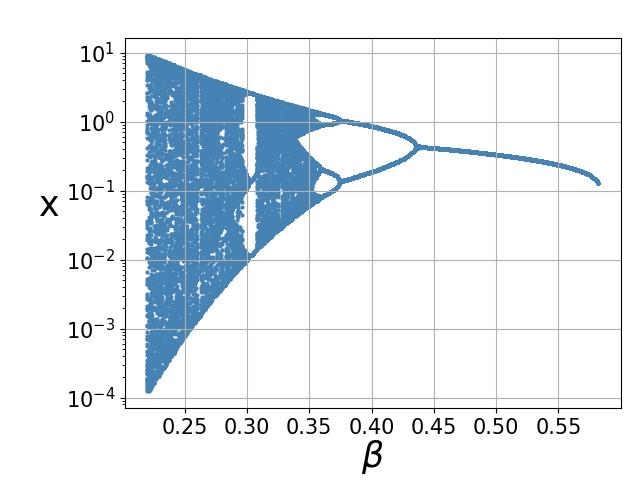
\includegraphics[width=\textwidth]{stochastic/images/bifurcation_x_0_2_a_1_compare_no_noise.jpg}
        
    %     \captionsetup{justification=centering}
    %     \caption{Бифуркационная диаграмма для модели (\ref{origin})}
    %     \label{bifurcation_x_0_2_a_1_compare_no_noise}
    % \end{figure}
